\documentclass[aspectratio=169]{beamer}
\usepackage{preamble_beamer}

\newcommand*{\QEDB}{\null\nobreak\hfill\ensuremath{\square}}

\newtheorem*{question*}{Вопрос}
\newtheorem*{claim*}{Утверждение}

\title[Американские опцион]{Семинар 6. Американские опционы} % The short title appears at the bottom of every slide, the full title is only on the title page

\begin{document}

\begin{frame}
\titlepage 
\end{frame}

\begin{frame}{Контракты американского типа}

    \begin{block}{Определение}
        Американский опцион с функцией выплатой $\Phi(t, S_t)$ -- контракт, 
        держатель которого может получить случайную сумму денег $\Phi(t, S_t)$ в произвольный момент времени $t \leq T$.
    \end{block}

    \begin{itemize}
        \item Выплата может произойти в произвольный момент времени.
        \item Стоимость европейского контракта:
        $$
            V_0^E = \E e^{-rT} \Phi(T, S_T)
        $$
        \item Стоимость американского контракта:
        $$
            V_0^A = \sup_{\tau \in \mathcal{T}} \E e^{-r\tau} \Phi(\tau, S_{\tau})
        $$
        \item $V_0^A$ -- стоимость реплицирующей стратегии.
        \item Дата погашения $\tau$ -- марковский момент $\{\tau \leq t\} \in \F_t$
        \item Принимаем решение об экспирации на основании информации из прошлого.    
    \end{itemize}
\end{frame}


\begin{frame}{Американские опционы: свойства}
    \begin{itemize}
        \item Оценка снизу:
        $$
            V_0^A \geq \max_{0\leq t \leq T} \E e^{-rt} \Phi(t, S_{t})
        $$В частности $V_0^A \geq V_0^E$, $V_0^A \geq \Phi(0, S_0)$.
        \item Оценка сверху:
        $$
            V_0^A \leq \E \max_{0 \leq t \leq T} e^{-rt} \Phi(t, S_{t})
        $$
    \end{itemize}
\end{frame}

\begin{frame}{Американский колл-опцион: свойства}
    \begin{itemize}
        \item Неравенство для европейского колл-опциона при $r>0$:
        \begin{align*}
            V_t^E &= \E\left[e^{-r(T-t)} (S_T - K)^+ | \F_t \right]
            \geq \left(\E\left[e^{-rT}(S_T - K)| \F_t \right]\right)^+ = \\
            &= (S_t - e^{-r(T-t)}K)^+ > (S_t - K)^+
        \end{align*}
        \item Отсюда $V_t^E \geq \Phi(t, S_t) \to V_t^A = V_t^E$
    \end{itemize}
\end{frame}

\begin{frame}{Бермудский опцион}
    \begin{block}{Определение}
Бермудский опцион с функцией выплатой $\Phi(t, S_t)$ -- контракт, 
        держатель которого может получить случайную сумму денег $\Phi(t, S_t)$ 
        в один из дискретных моментов времени $t\in\{t_1, t_2, \ldots, t_n\}$
    \end{block}

\end{frame}
\begin{frame}{Бермудский опцион: уравнение на цену}
    \begin{itemize}
        \item Стоимость бермудского контракта:
        $$
            V_0^B = \sup_{\tau \in \overline{\mathcal{T}}} \E e^{-r\tau} \Phi(\tau, S_{\tau})
        $$где $\overline{\mathcal{T}}$ -- множество моментов остановки со значениями из $\{t_1, \ldots, t_n\}$.
        \item $V_{t_k}^B$ -- стоимость бермудского опциона в момент $t_k$ при условии, что не экспирировались до момента $t_k$.
        \item Continuation value -- стоимость, при условии что не экспирируемся в $t_k$:
        $$
            C_{t_k} = \E\left[ e^{-r \Delta t_k} V_{t_{k+1}}^B | \F_t \right]
        $$
        \item Динамическое программирование:
        $$
            V_{t_k} = \max(\Phi(t_k, S_{t_K}), C_{t_k})
        $$
        \item Оптимальный момент остановки:
        $$
            \tau = \inf\{t_k : \Phi(t_k, S_{t_K}) > C_{t_k} \}
        $$
    \end{itemize}
\end{frame}

\begin{frame}{Бермудский опцион: цены}
    \centering
    \makebox[\textwidth]{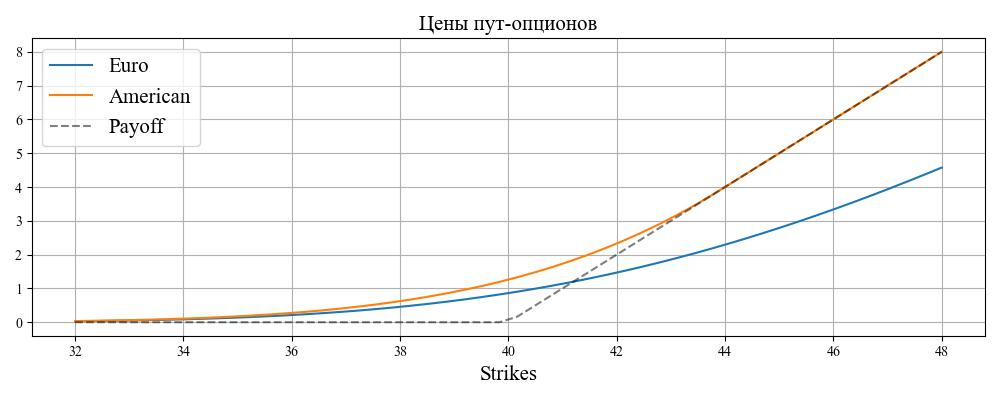
\includegraphics[width=1\textwidth]{6_figs/american_euro_prices.jpg}}
\end{frame}

\begin{frame}{Perpetual american put}
    \begin{block}{Задача}
        Найти стоимость вечного американского пут-опциона $T=\infty$:
        $$
            V(s) = \sup_{\tau \in \mathcal{T}} \E e^{-r\tau} (K-S_{\tau})
        $$где супремум берётся по всем марковским моментам $\mathcal{T}$, $S_0 = s$.
    \end{block}
\end{frame}

\begin{frame}{Perpetual american put}
    \begin{itemize}
        \item Задача однородная по времени. Ищем решение в классе моментов остановки:
        $$
            \tau_L = \inf\{t \geq 0, S_t = L\}
        $$
        \item Исполняем опцион в первый момент, когда цена пробъёт уровень $L < s$.
        \item Найдем ожидаемую выплату для такой стратегии:
        $$
            V_L(s) = \E e^{-r\tau_L}(K-S_{\tau_L})
            = (K-L)\E e^{-r\tau_L}
        $$Считаем, что $e^{-r\tau_L}(K-S_{\tau_L})=0$ при $\tau_L = \infty$ (выплаты не происходит).
        \item Нужно найти преобразование Лапласа от $\tau_L, \E e^{-r\tau_L}$.
    \end{itemize}
\end{frame}

\begin{frame}{Преобразование Лапласа}
    \begin{itemize}
        \item БД со сносом $X_t = \mu t + W_t$
        \item Моменты остановки 
        $\tau_a = \inf\{t \geq 0: X_t = a\}$,
        $\tau_b = \inf\{t \geq 0: X_t = -b\}$
        \item Найдем $\sigma$ такое, что $M_t$ -- мартингал:
        $$
            M_t = e^{\sigma X_t - r t}
        $$
        \item Для момента $\tau = \tau_a \land \tau_b$ выполнена теорема Дуба:
        $$
            1 = \E M_{\tau} = 
            \E e^{\sigma a - r \tau_a} \mathbb{I}(\tau_a \leq \tau_b)
            + \E e^{-\sigma b - r \tau_b} \mathbb{I}(\tau_a > \tau_b) 
        $$При $b\to \infty$ второе мат. ожидание стремится к нулю, откуда:
        $$
            1 = \E e^{\sigma a - r \tau_a} \mathbb{I}(\tau_a < \infty)
            = e^{\sigma a} \E e^{- r \tau_a}
        $$откуда
        $$
            \E e^{-r\tau_a} = e^{-\sigma a}
        $$
        \item При $\sigma = -\mu + \sqrt{\mu^2 + 2r}$ $M_t$ матрингал, поэтому:
        $$
        \E e^{-r\tau_a} = e^{-(-\mu + \sqrt{\mu^2 + 2r}) a}
        $$
    \end{itemize}
\end{frame}

\begin{frame}{Perpetual american put: продолжение}
    \begin{itemize}
    \only<1>{\item $X_t = \frac{1}{\sigma} \log \frac{S_t}{s} 
    = \frac{1}{\sigma}(r - 0.5 \sigma^2)t + W_t$
    \item $S_t = L \Leftrightarrow X_t = \frac{1}{\sigma}\log \frac{L}{s}$
    \item 
    $\E e^{-r\tau_L} = e^{-(-\mu + \sqrt{\mu^2 + 2r}) a}$, где $\mu = \frac{1}{\sigma}(r - 0.5 \sigma^2), 
    a = \frac{1}{\sigma}\log \frac{L}{s}$:
    $$
     \E e^{-r\tau_L} = \left(\frac{s}{L}\right)^{-\frac{2r}{\sigma^2}}
    $$}
    \only<1->{\item Итого, ожидание выплаты для такой стратегии:
    $$
        v_L(s) = \begin{cases} 
            K-s, 0 \leq s \leq L \\
            (K-L) \left(\frac{s}{L}\right)^{-\frac{2r}{\sigma^2}}, s \geq L
        \end{cases}
    $$
    \item Оптимальная граница $L$:
    $$
        \dfrac{\partial v_L(s)}{\partial L} = 0 \to L^* = \dfrac{2r}{2r + \sigma^2} K
    $$}
    \only<2>{
    \item При таком выборе $L$ производная по $s$ непрерывна (smooth pasting):
    $$
        \left.\dfrac{\partial v_{L^*}(s)}{\partial s} \right\vert_{L^*-0}
        = \left.\dfrac{\partial v_{L^*}(s)}{\partial s} \right\vert_{L^*+0}=-1
    $$}
    \end{itemize}
\end{frame}

\begin{frame}{Perpetual american put: цены}
    \centering
    \makebox[\textwidth]{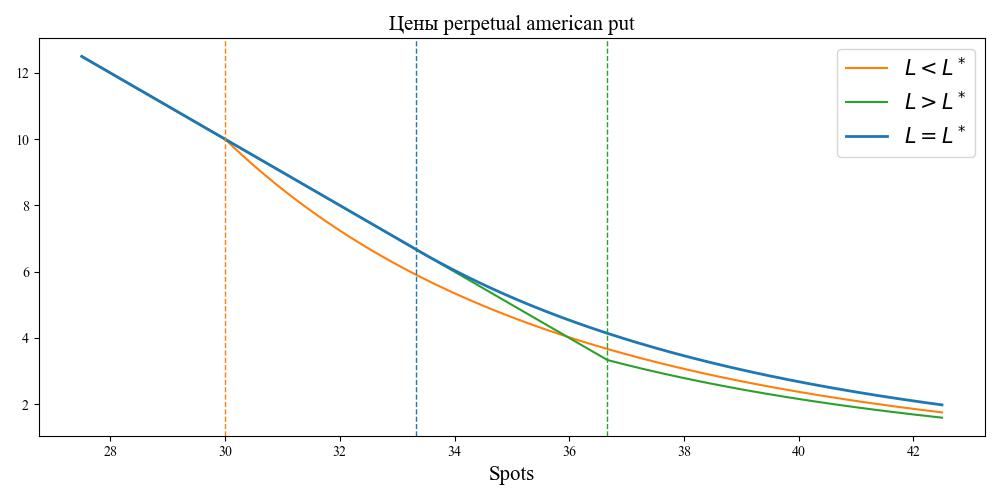
\includegraphics[width=1\textwidth]{6_figs/american_perpetual.jpg}}
\end{frame}

\end{document}
